 \section{Aufbau und Durchführung}
\label{sec:Durchführung}

\begin{figure}
  \centering
  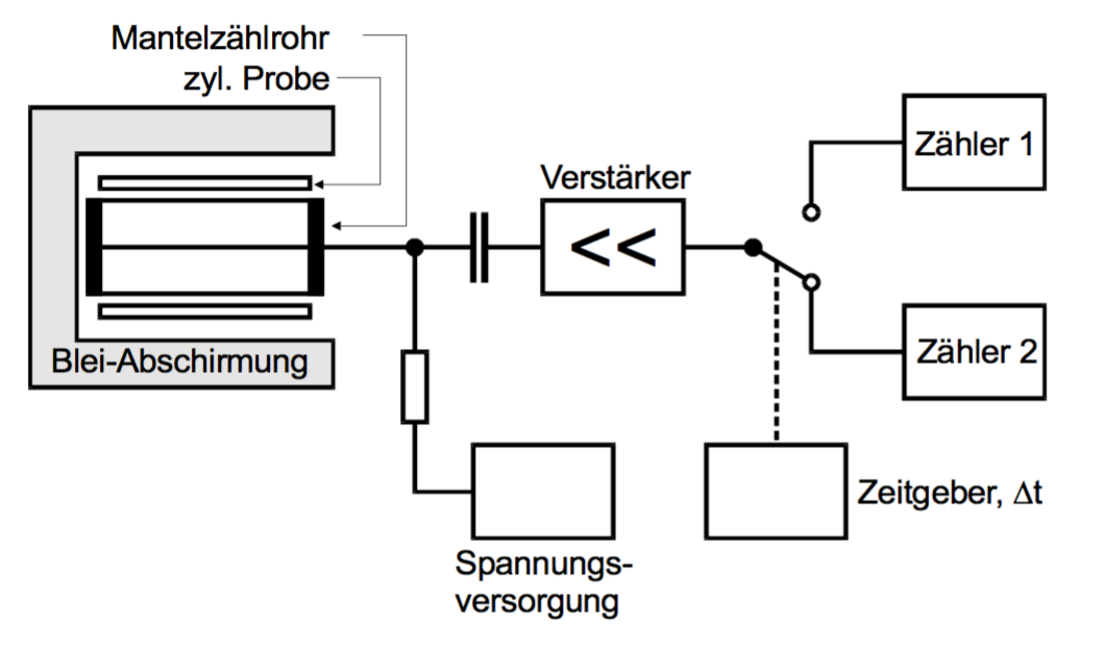
\includegraphics[width = \textwidth]{Pics/zaehleraufbau.pdf}
  \caption{Schematische Darstellung des Versuchsaufbaus.\cite{anleitung}}
  \label{fig:aufbau}
\end{figure}

In Abbildung \ref{fig:aufbau} zeigt sich wie die radioaktiven Zerfälle der Isotope
registriert werden. Das Geiger-Müller-Zählrohr nimmt in einem voreingestellten Zeitintervall
$\Delta t$ die abgestrahlten Impulse auf und zeigt sie an einem digitalen Zähler an.
Im nächsten Zeitintervall schaltet der in der Abbildung gezeigte Schalter die andere Anzeige
hinzu. So bleibt der Wert am ersten Zähler ein Zeitintervall lang stehen und es kann
entspannt abgelesen werden.

\begin{itemize}
  \item Die Aktivierung der Isotope wird im voraus durchgeführt. Die instabilen Isotope
  werden vom Behälter, in dem sie aktiviert werden,
  direkt in den Versuch eingebracht, um die Zerfallskurve in Gänze aufnehmen zu können.
  \item Zunächst wird eine Nullmessung durchgeführt, um zu bestimmen wie viel
  Umgebungsstrahlung detektiert wird. Dazu wird zwei Mal $\SI{900}{\second}$ ohne
  Probe gemessen.
  \item Dann wird eine 40 minütige Messung mit Jod durchgeführt. $\Delta t$
  beträgt hier $\SI{200}{\second}$.
  \item Die Messung mit Rhodium dauert zwölf Minuten mit $\Delta t = \SI{20}{\second}$.

\end{itemize}
